
It's not always possible to use derivative in order to optimize a
fonction with a continuous domain because:
\begin{enumerate}
    \item  The gradient is not computable
    \item  We dont know the objective function
    \item  The gradient is to expensive to compute
    \item  We don't know how to compute the gradient
\end{enumerate}

In this case, we can use \textbf{Derivative free optimization}.
We dont know the objective function but we have comparison function that allows us to compare solutions.


\subsection{Background}

\subsubsection{Single-objective Optimization problem}
\begin{tabular}{m{6cm}m{6cm}}
    \begin{eqnarray*}
        \textrm{Optimize } & f(X)\\
        \textrm{subject to } & X \in \Omega\\
    \end{eqnarray*}
    &
    where $ \begin{cases}
        X = (x_1, ..., x_n)\\
        f: \Omega \rightarrow \mathbb{R}\\
        \Omega \subseteq \mathbb{R}^n
    \end{cases}$
\end{tabular}

\subsubsection{Feasible Region}

Only consider $\Omega \subseteq \mathbb{R}^n$ which define hyper-volume:
$$\forall_i \in 1,..., n: \Omega_i = [l_i, u_i]$$ 
where $l_i, u_i \in \mathbb{R} and l_i \leq u_i$

\subsubsection{Comparison function}
$$cmp(x_1, x_2) : \Omega^2 \rightarrow \mathbb{B}$$

\paragraph{Example}
\begin{itemize}
    \item Classical minimization: $(x_1, x_2) \Rightarrow f(x_1)\leq
        f(x_2)$
    \item Classical maximization: $(x_1, x_2) \Rightarrow f(x_1)\geq
        f(x_2)$
    \item Probabilistic minimization: $(x_1, x_2) \Rightarrow E[f(x_1)]\geq
        E[f(x_2)]$
    \item ...
\end{itemize}

\subsection{Grid Search}

As the domain is continuous and we can't compare every point:

\begin{tabular}{m{10cm}m{7cm}}
\begin{enumerate}
    \item Cut each dimension of the domain $\Omega$ in m
    \item Evaluate each one of these combination 
    \item Output the minimum

    \item[$\Rightarrow$]  We will always have $m^n$ evaluation,
        because we have $n$ dimensions that
we cut in $m$ parts.
\end{enumerate}
&
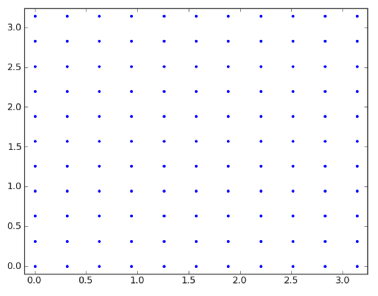
\includegraphics[width=4.5cm]{grid}
\end{tabular}

\subsubsection{Iteratively}
\begin{itemize}
    \item Perform a grid search for the domain $\Omega$ 
    \item Around the min point found define a new smaller domain
        $\Omega$ 
    \item[$\Rightarrow$] So if we do i iterations we will have $i *
        m^n$ evaluations for the objective.
\end{itemize}

\subsection{Directional Direct Search}

\begin{tabular}{m{12cm}m{3cm}}
The global idea is to \textbf{test a sample of points} in specified
directions around the iterate.
If a point is better, select it as next iterate.
&

\includegraphics[width=2cm]{DDS}
\end{tabular}

\subsubsection{Step}

\begin{enumerate}
    \item \textbf{Poll step}: Test $N$ points in specified directions
        around iterate and stop when better (with our comparison
        function) point found.

        \begin{itemize}

            \item \textbf{Directions and bases}
                We define a set $D$ of positive bases used to evaluate new
                points (directions):
                $$D = [l, -l] = [e_1,..., e_n, -e_1,..., -e_n]$$
                where the $e_i (1 < i < n)$ are unit vector ($||e_i|| = 1$)

            \item \textbf{Build new point}: 
                $$x_(new) = x+\alpha*d \quad \textrm{where } d \in D$$
        \end{itemize}

        \paragraph{Example} For a 3D space,
        $$D = [l, -l] = [e_1, e_2, e_3, -e_1, -e_2, -e_3] \quad
        \textrm{where} \quad \begin{cases}
            e_1 = (1,0,0) \\
            e_2 = (0,1,0)\\
            e_3 = (0,0,1)\\
        \end{cases} $$
        $$\textrm{Suppose} \quad \begin{cases} 
            x = (40, 42, 42)\\
            d = (1, 0, 0)\\
            \alpha =2
        \end{cases} \quad           
        x_{new}  = (40, 42, 42) + 2 * (1, 0, 0) = (42, 42, 42)$$


    \item \textbf{Mesh parameter update}: Update or maintain the step
        size parameter, $\alpha_k$ in order to converge faster.

        \begin{enumerate}
            \item Iteration declared successful: increase $\alpha_k$ to
                perform greater step
                $$\alpha_{k+1} = \gamma \alpha_k \quad \textrm{with}\quad \gamma > 1$$

            \item Iteration declared unsuccessful: decrease $\alpha_k$ to
                converge to an optimum
                $$\alpha_{k+1} = \beta \alpha_k \quad \textrm{with}\quad
                0 < \beta < 1$$
            \end{enumerate}
\end{enumerate}

\subsubsection{Denis-Wood Coutours}

\begin{tabular}{m{12cm}m{5cm}}
No convergence if Denis-Wood contours appears in objective
function
&
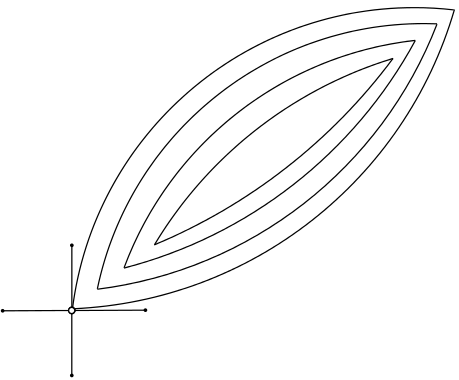
\includegraphics[width=2cm]{contour}
\end{tabular}

\paragraph{Two solutions}:
\begin{enumerate}
    \item Rotate the bases after $N$ unsuccessful iterations
    \item Run DDS $N$ times with $N$ different set of bases.
    \end{enumerate}

\subsubsection{One iteration complexity}
\begin{itemize}
    \item Worst case: $Nb_{evals} = 2b = 0(b)$ where $b$ is the number
        of bases used
    \item Best case: $Nb_{evals} = 1 = \Omega(1)$
\end{itemize}


\subsection{The Nelder-Mead Algorithm}

The global idea is to build a structure of points and replace the worst
point at each iteration.

\subsubsection{Simplex}
\begin{tabular}{m{12cm}m{3cm}}
    \begin{itemize}
        \item The structure of point is a polyhedron of dimension $n+1$
            (abusively called simplex)

    \item The simplex structure $Y$ is a set of $n+1$ vertices where $n$ is the
dimension of the search space defined as follows:
$$Y = \{y^0,y^1,...,y^n\}$$

\item The vertice $y^0$ is a better solution than the vertice $y^1$ which is a better solution that then vertice $y^2$ ....
        \end{itemize}
&
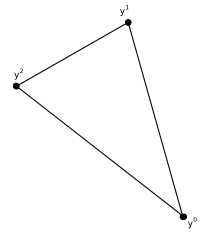
\includegraphics[width=3cm]{polyhedron}
\end{tabular}

\subsubsection{Operations on the simplex}
At each iteration, replace the worst point by performing one of the
following actions:
\begin{enumerate}
    \item \begin{tabular}{m{9cm}m{3cm}}
            \textbf{Reflection} if $f^0 \leq f < f^{n-1}$ : Replace $y^n$ by $y^r$

            $$Nb_{evals} = 1 = \Theta(1)$$
            & 
            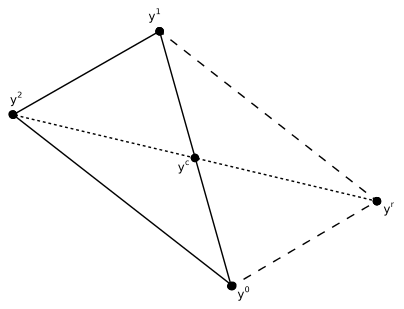
\includegraphics[width=4cm]{reflection}
        \end{tabular}

    \item \begin{tabular}{m{9cm}m{3cm}}
            \textbf{Expansion} if $f^r < f^0$ : 
            \begin{itemize}
                \item If $f^e \leq f^r$ replace $y^n$ by $y^e$
                \item else replace $y^n$ by $y^r$
            \end{itemize}

            $$Nb_{evals} = 2 = \Theta(1)$$
            & 
            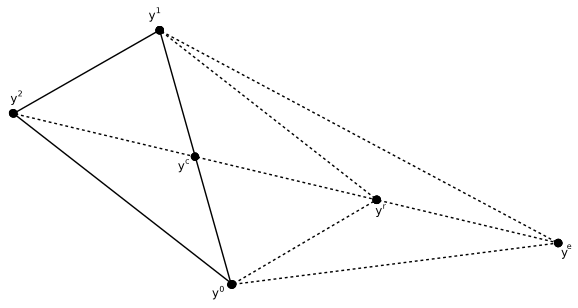
\includegraphics[width=4cm]{expansion}
        \end{tabular}

    \item \begin{tabular}{m{9cm}m{3cm}}
            \textbf{Contraction} if $f^r \geq f < f^{n-1}$ : 
            \begin{itemize}
                \item If $f^r < f^n$ replace $y^n$ by $y^{oc}$ (outside)
                \item else replace $y^n$ by $y^{ic}$ (inside)
            \end{itemize}

            $$Nb_{evals} = 2 = \Theta(1)$$
            & 
            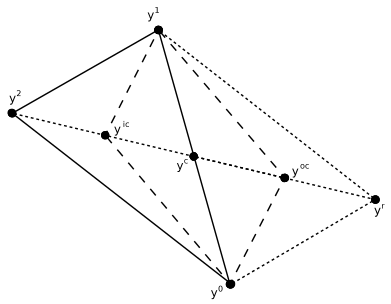
\includegraphics[width=4cm]{contraction}
        \end{tabular}

    \item \begin{tabular}{m{9cm}m{3cm}}
            \textbf{Shrink} if no amelioration by doing thos 

            $$Nb_{evals} = n+2 = \Theta(n)$$ where $n$ is the dimension
            of the search space
            & 
            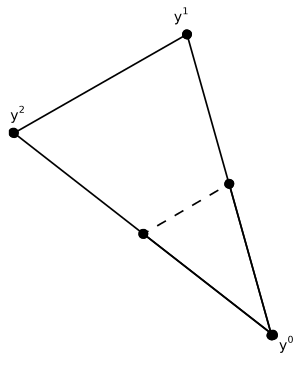
\includegraphics[width=4cm]{shrink}
        \end{tabular}
\end{enumerate}


\subsection{Multi-Directional Search}

Globally, it's the same point structure than in Nelder-Mead.
\begin{itemize}
    \item Perform operations on all but one vertices of the simplex around
        the best vertex.

    \item The structure of point is a polyhedron of dimension n + 1 (The
        simplex of Nelder-Mead).
\end{itemize}

\subsubsection{Operations on the simplex}
$$\textrm{Evaluate }: f^r = min \{ f(y_i^r) | i=1,...,n\}$$
\begin{enumerate}
        %TODO
    \item \begin{tabular}{m{9cm}m{3cm}}
            \textbf{Rotation } 

if $f^r$ < $f^0$ -> expansion\newline
else -> contract simplex \newline


            $$Nb_{evals} = n = \Theta(n)$$ where $n$ is the dimension
            of the search space
            & 
            %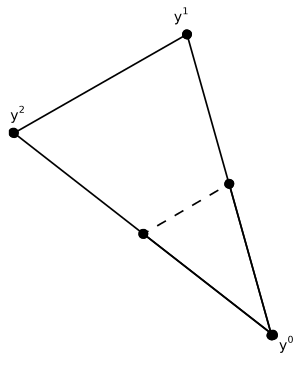
\includegraphics[width=4cm]{shrink}
        \end{tabular}

    \item \begin{tabular}{m{9cm}m{3cm}}
            \textbf{Expansion } 

if $f^e$ < $f^r$ -> The new simplex is the expanded simplex\newline
else -> cThe new simplex is the rotated simplex \newline

            $$Nb_{evals} = 2b = \Theta(n)$$ where $n$ is the dimension
            of the search space
            & 
            %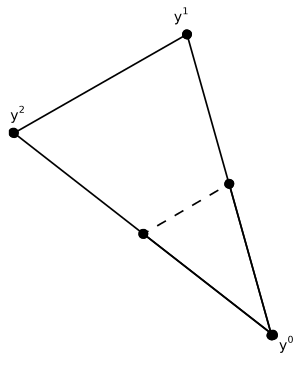
\includegraphics[width=4cm]{shrink}
        \end{tabular}

    \item \begin{tabular}{m{9cm}m{3cm}}
            \textbf{Shrink} if no amelioration by doing thos 

            $$Nb_{evals} = 2n = \Theta(n)$$ where $n$ is the dimension
            of the search space
            & 
            %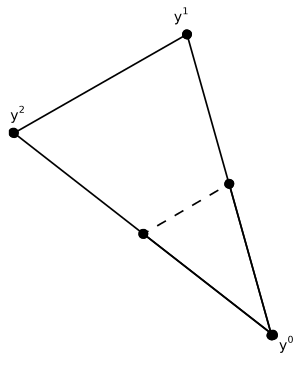
\includegraphics[width=4cm]{shrink}
        \end{tabular}
\end{enumerate}



\subsection{Smart Random Algorithms}
\begin{itemize}
    \item Problem: Algorithm might convert to local minimum.
    \item Solution:  Restart from different points
\end{itemize}

\subsubsection{Random restarts}
\begin{itemize}
    \item Run $N$ times the algorithm such as:
        \begin{enumerate}
            \item For each run the algorithm begins from a random starting
                point
            \item Random starting points following a uniform distribution
            \item Return the best result obtained over the N runs
        \end{enumerate}

    \item [$\Rightarrow $] With $N \rightarrow \infty $ we will
        eventually converge to a global optimum byt this take too much
        computation
\end{itemize}

\subsubsection{Halton sequence}

To perform better random sequence, we need to \textbf{reduce gaps
between point} which is the job of Halton sequence.

\begin{itemize}
    \item \textbf{Build 1D Halton sequence}
        \begin{enumerate}
            \item Choose a base (integer) 
            \item Successively decompose [0, 1]
                in subintervals according to the base.
        \end{enumerate}

        $$\textrm{Example base 2: } \frac{1}{2},
        \frac{1}{4},\frac{3}{4}, \frac{1}{8}, \frac{5}{8},
        \frac{3}{8}, \frac{7}{8}, ...$$

    \item \textbf{Build Multi-D Halton sequence}
        \begin{enumerate}
            \item Build $n$ 1D sequence with $n$ different bases (prime
                two by two)
            \item Mix them to build point
        \end{enumerate}


        $$\textrm{Example : } \Bigg[(\frac{1}{2}, \frac{1}{3}),
            (\frac{1}{4}, \frac{2}{3}), (\frac{3}{4}, \frac{1}{9}), (\frac{1}{8},
        \frac{4}{9}),(\frac{5}{8}, \frac{7}{9})\Bigg]    \quad
        \textrm{from } \quad
        \begin{cases}
            \frac{1}{2}, \frac{1}{4},\frac{3}{4}, \frac{1}{8}, \frac{5}{8}\\
            \frac{1}{3}, \frac{2}{3},\frac{1}{9}, \frac{4}{9}, \frac{7}{9}
        \end{cases}$$

\end{itemize}


\paragraph{Problem} With higher prime sequence, there is a correlation
problem.

\begin{itemize}
    \item[$\Rightarrow$] The solution is to \textbf{shuffle} all 1D sequences before
        mix them to build points 
\end{itemize}

